% !Mode:: "TeX:UTF-8"

\chapter[遗传算法并行化]{遗传算法并行化}
\section{遗传算法}
\subsection{遗传算法介绍}
    遗传算法是计算数学中用于解决最佳化的搜索算法,属于进化算法,由1960年于I.Rechenberg提出。进
化算法最初是借鉴了进化生物学的一些现象发展起来的,这些想象包含了遗传,突变,自然选择以及杂交等等。
遗传算法可以解决大部分问题,虽然不可能找到最优解,但是很多情况下,能够获得局部的最优解.
    
    遗传算法的核心思想如下:在求解一个问题最优解时,以一定数量的候选个体开始,向更好的种群进化。进化从
完全随机个体的种群开始,一代代的进化。在每一代中,整个种群的适应读被评价,从当前种群中随机地选择多个个体
,之后通过自然选择和突变产生新的生命群体,如果产生的新生命群体更为优秀,则该种群在算法的
下一次迭代中成为当前种群.

    遗传算法的核心在于寻找良好的适应度函数,遗传算法本身具有良好的简洁性和优秀的鲁棒性,n
能够在足够短的时间内获得到不错的效果.通常遗传算法适用于以下几个问题类型:

    \begin{itemize}
    \item 搜索空间非常大,问题过于复杂,难于被理解
    \item 专家知识太难,或者专家语言太难以编码搜索空间
    \item 没有可用的数学解
    \item 传统搜索方法不可用
    \end{itemize}

    遗传算法的非常适合处理有各种常量的问题,或者适合用权重等适应函数进行选择的问题,具体的应用领域有:

    \begin{itemize}
    \item 优化:遗传算法应用在了很多优化任务上,比如说数字归约优化,组合数优化,比如说旅行售货员
问题,电路设计,音视频质量优化等问题
    \item 自动问题:如网络规划,细胞分裂等问题
    \item 机器学习:例如自动分类,预测,蛋白质结构预测
    \item 经济模型:创新性的经济模型,竞价策略,经济市场的判断
    \item 人类基因模型:基因的重新组合规划
    \item 
    \end{itemize}

    遗传算法已经证明了其自身尅在许多复杂的领域中发挥自己的作用,具有良好的是适应性,能够应对和处理不同的方面
通过并行化的应用可以有效和隐式地降低多个独立生物代的创造时间,进一步优化算法效率.
    
\subsection{旅行售货员问题}
    旅行售货员问题内容为:有许多城市,城市之间有相连的道路,旅行售货员必须访问所有的城市,但是
他不怎么喜欢旅行,所以想寻找一条总路径最短的旅行方法.可以理解为具有N个结点的汉密尔顿回路.

    旅行售货员问题(Traveling Salesman Problem)可以使用遗传算法来解决,其本身是一个NP难的问题,在1930年被提出,可以被应用在
行程优化,逻辑规划,微芯片的制造.其本身已经被用作许多优化算法的测试基准,同时TSP已经获取到了许多
精确和优秀的解,可以解决书以十万计的城市.TSP问题可以在DNA排序里做为一个子问题,城市可以用来代
表结合位点,DNA结合为点,概念上的距离可以理解为履行时间或者花

\section{算法}

    遗传算法的步骤可以解释为
    \begin{enumerate}
    \item 初始化 $t\leftarrow0$ 初始化进化代数计数器;T 最大进化代数;随机生成M个个体做为初始群体P(t)
    \item 个体评价  计算P(t)中各个个体的适应度值
    \item 选择运算  将选择算子作用于群体,从原种群中获取父母(具有更好适应性的父母将被有限选择)
    \item 交叉运算  将交叉算子作用于群体,用于生成新的种群,
    \item 变异运算  将编译算子作用于群体,并通过一上运算得到下一代群体P(t+1);
    \item 判断运算  如果新一代的群体更加适合环境,则替换原群体.
    \item 终止条件判断 
    \end{enumerate}

    初始化 c1 1101100100110110
            c2 1101111000011110
    交叉  c1 11011 00100110110
            c2 11011 11000011110
            offspring1 11011 11000011110
            offspring2 11011 00100110110
    变异  o1  1101111000011110
            o2  1101100100110110
            mo1 1100111000011110
            mo2 1101101100110110

    遗传算法常见算法流程,如图~\ref{fig:genetic}所示,

    \begin{figure}[htbp]
    \centering
    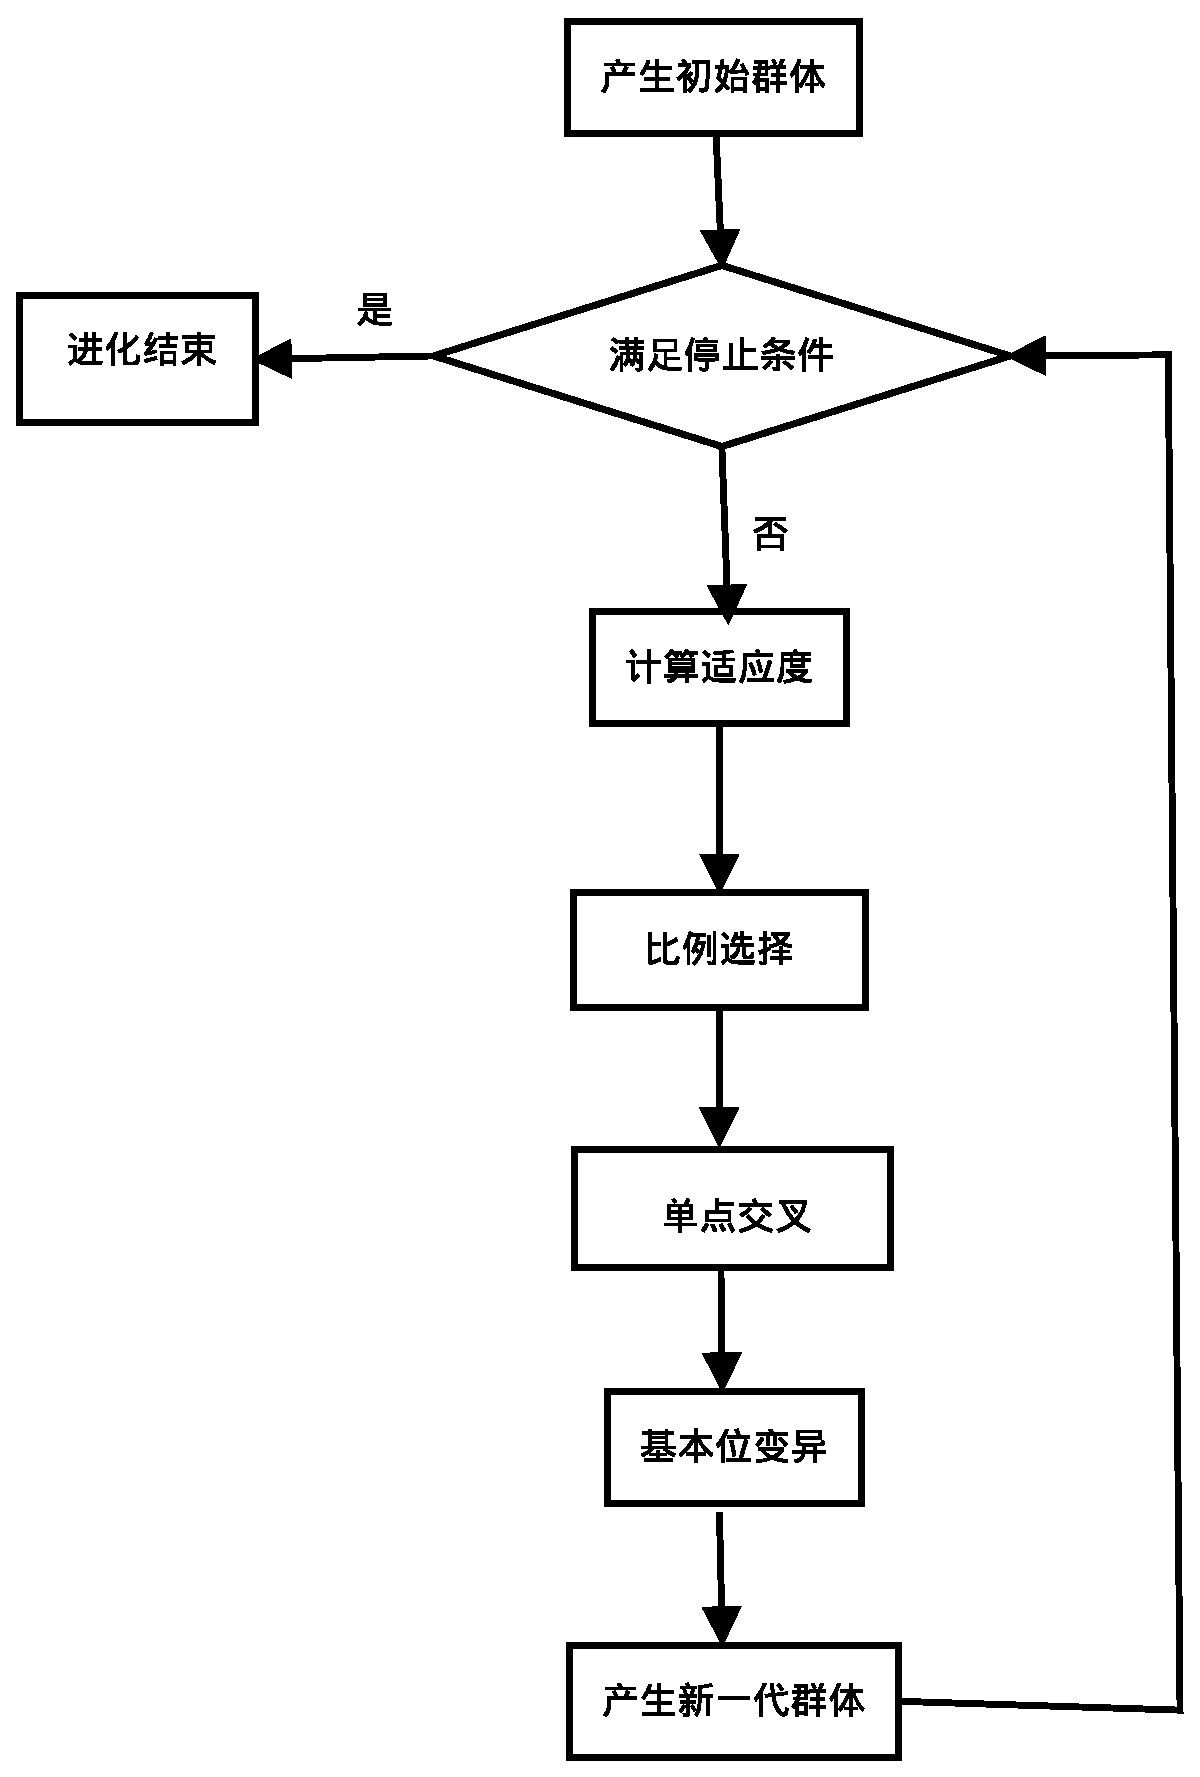
\includegraphics[width=0.4\textwidth]{genetic}
    \caption{遗传算法}\label{fig:genetic}
    \vspace{\baselineskip}
    \end{figure}

            
\section{算法伪代码}
\begin{algorithmic}
    \While{$\ell/N > threshold $}
    \State $\ell \gets 0$
    \For {$i \gets 0 , N-1 $}
        \For {$j \gets ,   K-1 $}
        \State  $   distance \gets |objects[i]-clusters[j]|$ 
        \If{$ distance < d_{min}$} 
        \State  $ d_{min} \gets distance $
                \State $n \gets j$
            \EndIf    
        \EndFor
        \If {$membership[i] \not= n $}
            \State $\ell \gets \ell + 1$
            \State $ membership[i] \gets n$
        \EndIf
       \State $newclusters[n] \gets newclusters[n]+objects[i] $
       \State $newclustersize[n] \gets  newclustersize[n]+$1
    \EndFor
    \For{$j \gets 0 ,K-1$}
       \State $clusters[j][*] \gets newclusters[j][*]/newclustersize[i] $
       \State $newclusters[j][*] \gets 0 $
       \State $newclustersize[j] \gets 0$
    \EndFor 
    \EndWhile
\end{algorithmic}

\section{实验结果}



%www.obitko.com/tutorials/genetic-algorithms/recommendations.php
